\placelogofalse
\begin{frame}{Multi-Level Intermediate Representation (MLIR)}
\begin{columns}
\column{0.58\linewidth}
\centering
\begin{outline}
  \1 Re-useable and Extensible Compiler Infrastructure
  \2 Chris Lattner + LLVM contributors
  \1 Focus on data-flow and computational kernels
  \2 LLVM IR is based on SSA machine
  \1 MLIR is based on dialects and passes
  \2 LLVM IR can be expressed as MLIR dialect
  \2 Targer accelerator specific instructions
  \2 Highly extensible
  \2 AND
  \2 Batteries includes
\end{outline}

\column{0.38\linewidth}
\begin{center}
\centering
\shadowimage[width=4.5cm]{mlir_paper.png}

%\includegraphics[width=2.5cm]{example_3.png}

% [trim={left bottom right top},clip]
%
\includegraphics[width=8.5cm, page=3, trim={0 9cm 14cm 0cm},clip]{assets/vec_db_figs.pdf}
\end{center}
\end{columns}
\end{frame}
\placelogotrue

\placelogofalse
\begin{frame}{MLIR for Direct Solvers}
\begin{columns}
\column{0.48\linewidth}
\centering
\begin{outline}
  \1 Includes Affine space representation
  \2 Polyhedral compilation
  \2 Tiling
  \1 Can target CPU / GPU / ect.
  \1 Focus on Compute Kernels
\end{outline}

\column{0.48\linewidth}
\begin{center}
\centering


%\shadowimage[width=2.5cm]{example_1.png}

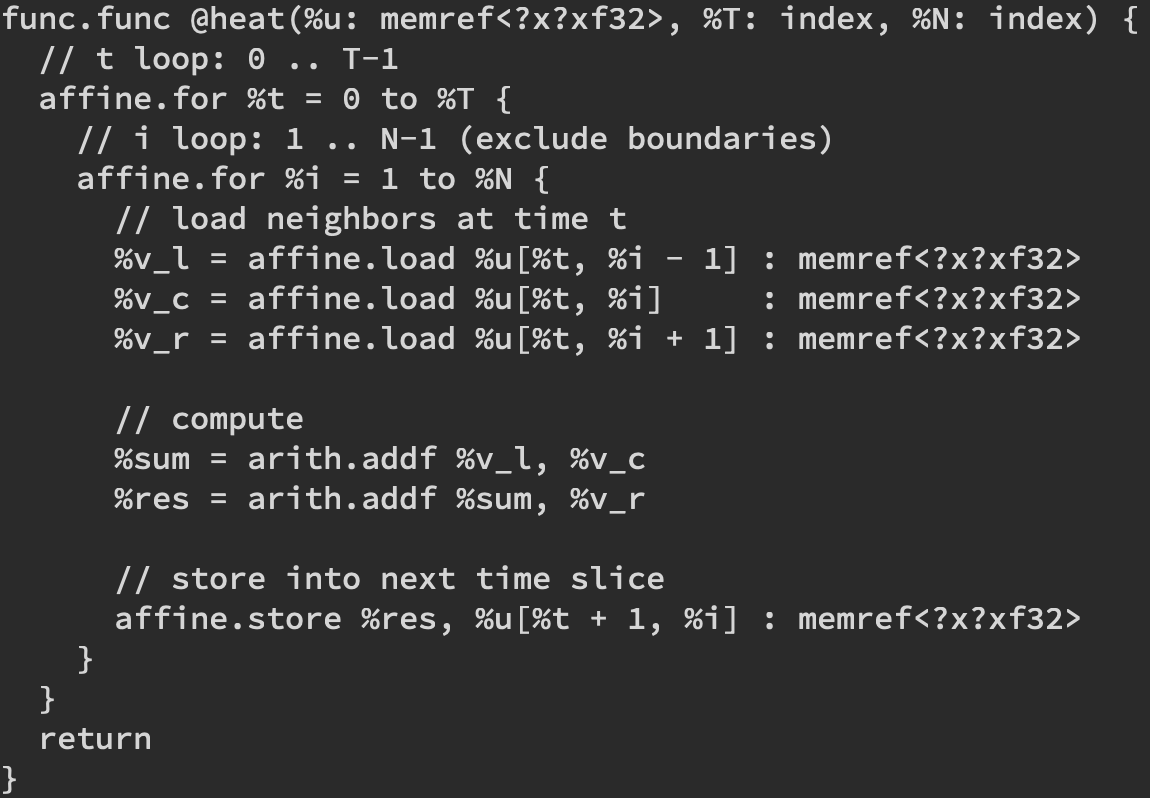
\includegraphics[width=4.5cm]{mlir_heat.png}

\vspace{0.3cm}

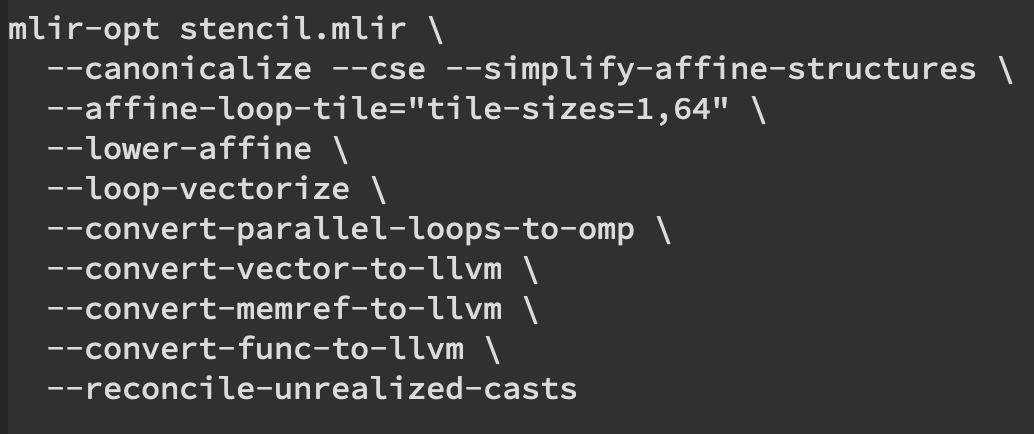
\includegraphics[width=5.0cm]{mlir_passes.png}

% [trim={left bottom right top},clip]
%
\includegraphics[width=8.5cm, page=3, trim={0 9cm 14cm 0cm},clip]{assets/vec_db_figs.pdf}
\end{center}
\end{columns}
\end{frame}
\placelogotrue
